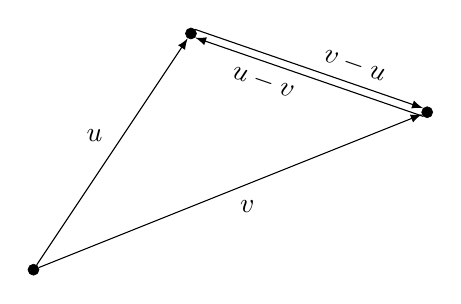
\begin{tikzpicture}[
	point/.style={circle,draw,very thin,fill,inner sep=0pt,minimum size=4pt},
	vector/.style={-latex},
]
	\node[point] at (0,0) (p) {};
	\node[point] at (2,3) (q) {};
	\node[point] at (5,2) (r) {};
	\draw[vector] (p) to node[above left] {$\uvec{u}$} (q);
	\draw[vector] (p) to node[below right] {$\uvec{v}$} (r);
	\draw[vector] (r.south west) to node[below left,sloped] {$\uvec{u}-\uvec{v}$} (q.south east);
	\draw[vector] (q.north east) to node[above right,sloped] {$\uvec{v}-\uvec{u}$} (r.north west);
\end{tikzpicture}
